\documentclass{article}
\usepackage{spconf}
\usepackage[T1]{fontenc} 
\usepackage[utf8]{inputenc}

\usepackage{algorithm}
\usepackage{algpseudocode}
\usepackage{color}
\usepackage[usenames,dvipsnames]{xcolor}
\usepackage[bookmarks=false, hidelinks]{hyperref}
\usepackage{graphicx}
\usepackage[tableposition=top]{caption}
\usepackage{subcaption}
\usepackage{amsmath}
\usepackage{amssymb}
\usepackage{breqn}
\usepackage{pgfplots}
\usepackage{tikz}
\usepackage{array}
\usepackage{hhline}
\usepackage{numprint}

\usetikzlibrary{matrix}
\usetikzlibrary{arrows}


\usepackage{mathtools}
\DeclarePairedDelimiter{\floor}{\lfloor}{\rfloor}
\DeclarePairedDelimiter{\ceil}{\lceil}{\rceil}

\hypersetup{
    colorlinks=true,
    linkcolor=black,
    citecolor=black,
    filecolor=black,
    urlcolor=black,
}

\hyphenpenalty=5000
\tolerance=1000

\newcommand{\beq}{\begin{dmath}}
\newcommand{\eeq}{\end{dmath}}
\newcommand{\beqs}{\begin{aligned}}
\newcommand{\eeqs}{\end{aligned}}

\newcommand{\x}{\mathbf{x}}
\newcommand{\hx}{\hat{\mathbf{x}}}
\newcommand{\B}{\mathbf{b}}
\newcommand{\R}{{R(\x)}}
\newcommand{\C}{\mathbf{c}}
\newcommand{\D}{D_p(\x)}
\newcommand{\SAD}{\text{SAD}}
\newcommand{\mGolomb}{G}
 
\newcommand{\vc}{\mathbf{c}}
\newcommand{\vx}{\mathbf{x}}
\newcommand{\vy}{\mathbf{y}}

\newcommand{\LM}{\lambda_{\text{\tiny{MOTION}}}}

\title{Rate Distortion-Based Motion Estimation Search Ordering For Rate-Constrained Successive Elimination Algorithms}
\name{Luc Trudeau, St\'ephane Coulombe, Christian Desrosiers\thanks{This work was funded by Vantrix Corporation and by the Natural Sciences and Engineering Research Council of Canada under the Collaborative Research and Development Program (NSERC-CRD 428942-11). Emails: luc.trudeau.1@ens.etsmtl.ca, \{stephane.coulombe, christian.desrosiers\}@etsmtl.ca}}
\address{Department of Software and IT Engineering\\ \'Ecole de technologie sup\'erieure, Universit\'e du Qu\'ebec\\ Montr\'eal, Qu\'ebec, Canada}

\begin{document}

\maketitle

\begin{abstract}
\vspace{-0.1em}
In this paper, we propose a new class of search ordering algorithms to reduce
the computational cost of motion estimation in video coding. We show that
conventional search orderings, such as spiral search, can weaken the filtering
criterion of rate-constrained successive elimination algorithms. Based on this
new insight, we derive a new search ordering that takes into account the impact
of the rate constraint. Our simulation results demonstrate that, on average, the
amount of SAD operations required to encode the tested sequences, is reduced
by 2.86\%, when compared to the H.264 JM reference software's implementation of
spiral search. For sequences with unpredictable motion, this reduction is greater than
5\% and can exceed 10\% when smaller block partitions are evaluated.
\end{abstract}

\begin{keywords}
\small{Successive elimination algorithm, motion estimation, H.264, Lagrange multiplier}
\end{keywords}

\vspace{-0.5em}
\section{Introduction}
\vspace{-0.2em}
\label{sec:intro}
Motion estimation is a predominant task of most modern video encoders. In the
H.264 video encoding standard~\cite{Wiegand2003}, when motion estimation is used
to encode a frame, it is performed on every non-overlapping $16\!\times\!16$
block. These blocks are called \textit{current blocks}. Motion estimation is
also performed inside the current block, for partitions of sizes $16\!\times\!16,
16\!\times\!8, 8\!\times\!16, 8\!\times\!8, 8\!\times\!4, 4\!\times\!8, 4\!\times\!4$.
Motion estimation consists of finding an optimal matching block in a search area
of size $(2W+1)\times(2W+1)$, where $W$ is the full pel length of the search
area. The blocks inside this search area are called \textit{candidate blocks},
and the search area can span over multiple reference frames, and up to quarter
pel precision is supported.

An exhaustive search algorithm (ESA) will obtain an optimal match by evaluating
each candidate block inside the search area. The high computational complexity
incurred by evaluating the cost function for all possible candidate blocks
allowed in H.264 limits practical applications of ESA in modern encoders. Many
algorithms reduce this computational complexity, and can be classified by
whether or not they preserve optimality. Algorithms that do not preserve
optimality often rely on the assumption of a monotonically increasing match
criterion around the location of the optimal candidate block. When this
assumption does not hold, accuracy of the motion estimation is reduced, as it
will converge to a local minimum. Modern algorithms in this class include
zonal search algorithms \cite{Tourapis2000, Tourapis2002}, which 
first evaluate a set of predictors in order to constrain a local diamond or
square search to a very narrow part of the search area.

Optimality preserving algorithms often rely on known inequalities, to avoid
computing the cost function of candidate blocks during the search process.
Recent algorithms in this class append more efficient filtering criteria to the
successive elimination algorithm (SEA) proposed in~\cite{Li1995a}. For example,
\cite{Gao2000, Zhu2005a} in their own way propose the use of partitions inside
blocks to improve filtering efficiency.

In~\cite{Coban1998a}, Coban and Mersereau modified the SEA to take into account
the number of bits required to encode the motion vector of a candidate block, by
altering the SEA criterion into a rate-constrained filtering criterion. This
alteration is in line with the H.264 joint model reference
software~\cite{Lim2004} where the optimal matching candidate block is the best
rate-constrained match. H.264-based SEA algorithms have been proposed
in~\cite{Yang2004, Toivonen2004}.

Another way the filtering criterion can be improved is via the candidate block search
ordering used for motion estimation. Spiral search ordering is known to
outperform a raster search ordering, and evaluates better
candidate blocks earlier in the search process, which in turn improves the filtering
criterion and allows more candidate blocks to be skipped. That is why the spiral
search ordering is used in many implementations of SEA-based
algorithms~\cite{Zhu2005a, Coban1998a, Yang2004}. This must however not to be confused
with SpiralPDE~\cite{Kim2000}, which is a spiral pattern used to sum the
elements of a block.

In this paper, we propose a new class of candidate block search ordering
algorithms, known as rate-constrained search ordering algorithms. We demonstrate
that conventional search ordering algorithms, such as raster and spiral search, can
impair the filtering criterion of rate-constrained successive elimination algorithms.
Rate-constrained search ordering algorithms do not lead to this impairment, making
them ideal for rate distortion contexts, like H.264 encoding.

This paper is organized as follows: In \autoref{sec:rdsea}, rate-constrained
successive elimination is described, and then the motivations for
rate-constrained search orderings are explained. We describe the proposed search
ordering in \autoref{sec:searchOrder}, which is derived from the
rate-constrained criterion used to filter candidate blocks. In
\autoref{sec:results}, experimental results for various sequences and
discussions of the results are given. Finally, \autoref{sec:conclusion}
concludes this paper.

\vspace{-0.5em}
\section{Rate-Constrained Successive Elimination Algorithms}
\label{sec:rdsea}
\vspace{-0.2em}
Successive Elimination Algorithms (SEA) are based on the following
inequality~\cite{Li1995a}
\vspace{-0.2em}:
\beq
| B - C(\vx_i,\vy_i) | \leqslant \SAD(\vx_i,\vy_i) \:,
\label{eq:SEA}
\eeq 
\vspace{-0.2em}
where $B$ is sum of the current block pixel values and $C(\vx_i,\vy_i)$ is the sum
of the pixel values of the $i$th candidate block located at position $(\vx_i,
\vy_i)$ in the search area. On the right hand side, the $\SAD(\vx_i,\vy_i)$
function returns the sum of the absolute differences between the pixel values of
the current block and those of the $i$th candidate block.

At first glance, the complexity of computing $B$ and $C(\vx_i,\vy_i)$ might seem
equivalent to that of computing the $\SAD(\vx_i,\vy_i)$ function, but that is
not the case, since Li and Salari~\cite{Li1995a} also proposed an apriori fast block
summation technique. During motion estimation, the values of $B$ and
$C(\vx_i,\vy_i)$ are obtained with table lookups, as shown on
lines~\ref{alg:RCSEA:Lookup1} and \ref{alg:RCSEA:Lookup2} of Algorithm
\ref{alg:RCSEA}. As explained in~\cite{Li1995a}, the overhead of
precaculating these sums is negligible and, overall, reduces computational costs
by 85\% when compared to ESA.

The filtering criterion works in the following manner: for a given candidate
block, if the left-hand side of equation~\eqref{eq:SEA}, a lower bound for
its SAD value, is higher than the current best SAD value of the search area,
then this candidate is not optimal. Therefore, the current best SAD value is used
as a threshold to decide when to avoid computing the SAD function.

The Rate-Constrained Successive Elimination Algorithms, originally proposed
by~\cite{Coban1998a}, states that to be optimal, the $i$th candidate block must
satisfy the following inequality:
\vspace{-0.2em}
\beq
\begin{aligned}
| B - &C(\vx_i,\vy_i) | + \lambda R(\vx_i,\vy_i) \\ \leqslant
& \SAD(\vx^*_{i-1},\vy^*_{i-1}) + \lambda R(\vx^*_{i-1},\vy^*_{i-1}) \:,
\end{aligned}
\label{eq:RDSEA}
\eeq 
\vspace{-0.2em}
where $\lambda$ is the Lagrange multiplier, a trade-off between rate and
distortion. Often referred to as rate, the $R(x,y)$ function returns the number
of bits required to encode the motion vector of the candidate block at position
$(x,y)$. The term $(\vx^*_{i}, \vy^*_{i})$ is the current best candidate block,
having considered the candidate blocks from 0 to $i-1$ in the scan ordering, and
is such that:
\vspace{-0.2em}
\beq
\begin{aligned}
\forall n \in \{0,\ldots,i\} & \Bigl( \SAD(\vx^*_{i},\vy^*_{i}) + \lambda
R(\vx^*_{i},\vy^*_{i}) \\ 
\leqslant & \: \SAD(\vx_{n},\vy_{n}) + \lambda
R(\vx_{n},\vy_{n})\Bigr)\:.
\end{aligned}
\eeq
\vspace{-0.2em}
It is important to note that the best candidate is no longer the lowest $\SAD$
value, but the best rate-constrained $\SAD$ value. 

Algorithm~\ref{alg:RCSEA} details the implementation of a motion estimation
algorithm enhanced with a rate-constrained successive elimination algorithm. 
\vspace{-0.5em}
\begin{algorithm}
\small{
\caption{Motion estimation algorithm enhanced with the rate-constrained
successive elimination algorithm.}
\label{alg:RCSEA}
\begin{algorithmic}[1]
\Function{MotionEstimation}{block, minCost}
\State $i^* \gets -1$ \Comment{negative when no better candidate is found}
\State $B\gets \text{sumB}[\text{block}.x][\text{block}.y]$
\label{alg:RCSEA:Lookup1}
\For{$i\gets 0 \text{ to numCand} $}
	\State $x\gets \text{ordering}[i].x$
	\State $y\gets \text{ordering}[i].y$
	
	\State $\text{cost} \gets \lambda \times R(x, y)$
	\If{$\text{cost} \geqslant \text{minCost}$}
		\State \textbf{return minCost}
	\EndIf
	\State $C\gets \text{sumC}[\text{block}.x + x][\text{block}.y + y]$
	\label{alg:RCSEA:Lookup2}
	\If{$|B - C| < \text{minCost} - \text{cost}$}
	\label{alg:RCSEA:Filtering}
		\State $\text{cost} \gets \text{cost} + \SAD(x,y)$
		
		\If{$\text{cost} < \text{minCost}$}
			\State $\text{minCost} \gets \text{cost}$
			\State $i^* \gets i$
		\EndIf
	\EndIf
\EndFor
\State \textbf{return} minCost, $i^*$
\EndFunction
\end{algorithmic}
}
\end{algorithm}
\vspace{-0.5em}
More precisely, sumB and sumC are lookup tables for the precalculated block
sums, ordering is a lookup table for candidate block ordering and minCost is the
cost of the current best candidate block. The filtering operation occurs on
line~\ref{alg:RCSEA:Filtering}, thus allowing the SAD function to be skipped if the
condition in~\eqref{eq:RDSEA} is not met.

One of the issues tackled by Coban and Mersereau~\cite{Li1995a} is finding the optimal value of
$\lambda$. This is somewhat resolved by the H.264 standard
recommendations~\cite{Lim2004}, as the recommended value of $\lambda$ can be
obtained with the following equation:
\beq
\LM = \left( w \times 2^{\left(\frac{QP - 12}{3}\right)}\right)\:, 
\eeq 
where $w$ varies from $0.65$ to $0.85$, depending on the type of frame that is
being encoded. This is somewhat a solution to the problem, but is in no way the
optimal value of $\lambda$.

Equation~\eqref{eq:RDSEA} can be written as follows:
\vspace{-0.2em}
\beq
\begin{aligned}
 | &B - C(\vx_i,\vy_i) | \\
  & \leqslant
\SAD(\vx^*_{i-1},\vy^*_{i-1}) + \lambda (R(\vx^*_{i-1},\vy^*_{i-1}) - R(\vx_i,\vy_i)) \:. 
\end{aligned}
\label{eq:InterestingForm}
\eeq
\vspace{-0.2em}

This form of the equation is interesting because of the difference between
$R(\vx^*_i,\vy^*_i)$ and $R(\vx_i,\vy_i)$. Let $\Delta R_i$ be the result of this
differentiation for the $i$th candidate block,
\vspace{-0.2em}
\beq
\Delta R_i = R(\vx^*_i,\vy^*_i) - R(\vx_i,\vy_i)\:.
\eeq
\vspace{-0.2em}
If $\Delta R_i$ is positive, then this will increase the filtering threshold
in~\eqref{eq:InterestingForm} by $\lambda\!\times\!\Delta R_i$ and thus weaken the
rate constraint on the filtering criterion.
This will often occur both in raster and spiral search ordering.

In the next section, we present a new class of search ordering algorithms that
do not weaken the rate-constrained filtering criterion.

\vspace{-0.5em}
\section{Rate-Constrained Search Ordering Algorithms}
\label{sec:searchOrder}
\vspace{-0.2em}
In light of the fact that the search ordering of candidate blocks can weaken a
rate-constrained filtering criterion, we propose a new class of candidate block
search ordering algorithms, known as rate-constrained search ordering
algorithms. To be classified as such, the ordering of the candidate blocks must
adhere to the following rule: the motion vector encoding cost of the current
candidate block must be equal to or greater than the preceding candidate block,
\vspace{-0.2em}
\beq
R(\vx_i, \vy_i) \geqslant R(\vx_{i-1}, \vy_{i-1})\:.
\label{eq:SearchOrdering}
\eeq
\vspace{-0.2em}
This guarantees that $\Delta R_i \leqslant 0$, thus never weakening the
rate constraint on the filtering criterion.

However, this class of search ordering algorithms is dependent on the encoding
scheme used for the motion vectors of candidate blocks. For the H.264 standard,
each component of a motion vector is coded using exponential Golomb codes and
quarter pixel precision, and thus
\vspace{-0.2em}
\beq
R(x,y) = \mGolomb(4x) + \mGolomb(4y)\:,
\eeq
\vspace{-0.2em}
where the $\mGolomb$ function returns the number of bits required to code a
given value with an exponential Golomb code. This function can be defined as
follows:
\vspace{-0.2em}
\beq
\mGolomb(x) = 2 \times \floor{\log_2(2|x| + 1)} + 1 \:.
\eeq
\vspace{-0.2em}

In \autoref{fig:ExpGolomb2D}, we present the motion vector encoding costs of
candidate blocks for a very small part of an H.264 motion estimation search area
centered on the H.264 predicted motion vector. Analyzing these costs, we notice
that for the same distance from the center $(0,0)$, candidate blocks located
near the diagonal ($\vx_i \approx \vy_i$) are more expensive than those near the
axis ($\vx_i \not\approx \vy_i$).
\begin{figure}[htb] \centering
\vspace{-0.2em}
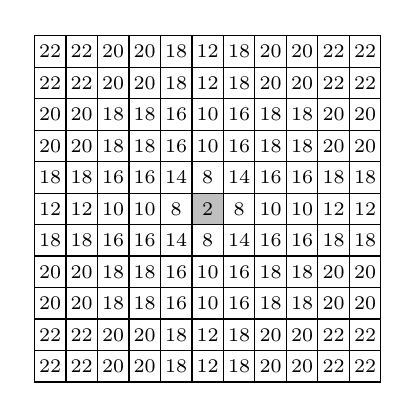
\begin{tikzpicture}

\tikzset{square matrix/.style={
    matrix of nodes,
    column sep=-\pgflinewidth, row sep=-\pgflinewidth,
    nodes={draw,
      minimum height=#1,
      anchor=center,
      text width=#1,
      align=center,
      inner sep=0pt
    },
  },
  square matrix/.default=0.4cm
}
\scriptsize{
\matrix[square matrix]{ & 22 & 22 & 20 & 20 & 18 &
12 & 18 & 20 & 20 & 22 & 22 \\ & 22 & 22 & 20 & 20 & 18 & 12 & 18 & 20 & 20 & 22 & 22 \\ 
& 20 & 20 & 18 & 18 & 16 & 10 & 16 & 18 & 18 & 20 & 20 \\
& 20 & 20 & 18 & 18 & 16 & 10 & 16 & 18 & 18 & 20 & 20 \\
& 18 & 18 & 16 & 16 & 14 &  8 & 14 & 16 & 16 & 18 & 18 \\
& 12 & 12 & 10 & 10 &  8 &  |[fill=lightgray]|2 &  8 & 10 & 10 & 12 & 12 \\
& 18 & 18 & 16 & 16 & 14 &  8 & 14 & 16 & 16 & 18 & 18 \\
& 20 & 20 & 18 & 18 & 16 & 10 & 16 & 18 & 18 & 20 & 20 \\
& 20 & 20 & 18 & 18 & 16 & 10 & 16 & 18 & 18 & 20 & 20 \\
& 22 & 22 & 20 & 20 & 18 & 12 & 18 & 20 & 20 & 22 & 22 \\
& 22 & 22 & 20 & 20 & 18 & 12 & 18 & 20 & 20 & 22 & 22 \\};
}
\end{tikzpicture}
\caption{ Grid of motion vector encoding bit lengths for the candidate blocks
of a search area. The center of the search area $(0,0)$ is the gray square.}
\label{fig:ExpGolomb2D}
\vspace{-0.2em}
\end{figure}
This helps to explain how the spiral search can weaken the rate-constrained
filtering criterion. If the current best candidate is close to or on the
diagonal, then the evaluation of candidate blocks closer to the axes will result
in a positive value for $\Delta R_i$, weakening the filtering criterion.

Applying the rule defined by equation~\eqref{eq:SearchOrdering} to the grid of
\autoref{fig:ExpGolomb2D} can result in multiple search orderings. In this paper,
we propose a search ordering that successively evaluates different quadrants
around the center $(0,0)$. The grids, \subref{fig:ProposedOrdering:Spiral} and
\subref{fig:ProposedOrdering:Proposed}, in \autoref{fig:ProposedOrdering} show
$5\!\times\!5$ subsets of the $65\!\times\!65$ grids tested in the next section.
\begin{figure}[htb] \centering
\vspace{-0.2em}
\begin{subfigure}{0.25\linewidth}
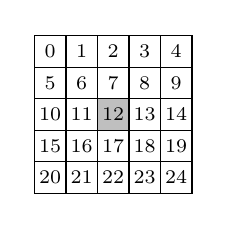
\begin{tikzpicture}

\tikzset{square matrix/.style={
    matrix of nodes, column sep=-\pgflinewidth, row sep=-\pgflinewidth,
    nodes={draw,
      minimum height=#1, anchor=center, text width=#1, align=center, inner
      sep=0pt
    },
  }, square matrix/.default=0.4cm
} \scriptsize{\matrix[square matrix]{ & 0 & 1 & 2 & 3 & 4 \\
& 5 & 6 & 7 & 8 & 9 \\
& 10 & 11 & |[fill=lightgray]| 12 & 13 & 14 \\
& 15 & 16 & 17 & 18 & 19 \\
& 20 & 21 & 22 & 23 & 24 \\};}
\end{tikzpicture}
\caption{}
\label{fig:ProposedOrdering:Raster}
\end{subfigure}
\begin{subfigure}{0.25\linewidth}
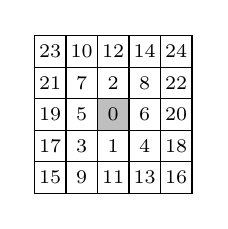
\begin{tikzpicture}

\tikzset{square matrix/.style={
    matrix of nodes, column sep=-\pgflinewidth, row sep=-\pgflinewidth,
    nodes={draw,
      minimum height=#1, anchor=center, text width=#1, align=center, inner
      sep=0pt
    },
  }, square matrix/.default=0.4cm
} \scriptsize{\matrix[square matrix]{ & 23 & 10 & 12 & 14 & 24 \\
& 21 & 7 & 2 & 8 & 22 \\
& 19 & 5 & |[fill=lightgray]|0 & 6 & 20 \\
& 17 & 3 & 1 & 4 & 18 \\
& 15 & 9 & 11 & 13 & 16 \\};}
\end{tikzpicture}
\caption{}
\label{fig:ProposedOrdering:Spiral}
\end{subfigure}
\begin{subfigure}{0.25\linewidth}
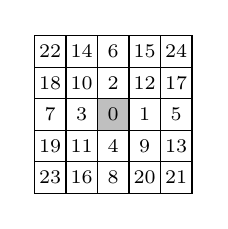
\begin{tikzpicture}

\tikzset{square matrix/.style={
    matrix of nodes, column sep=-\pgflinewidth, row sep=-\pgflinewidth,
    nodes={draw,
      minimum height=#1, anchor=center, text width=#1, align=center, inner
      sep=0pt
    },
  }, square matrix/.default=0.4cm
} \scriptsize{\matrix[square matrix]{ & 22 & 14 & 6 & 15 & 24 \\
& 18 & 10 & 2 & 12 & 17 \\
& 7 & 3 & |[fill=lightgray]|0 & 1 & 5 \\
& 19 & 11 & 4 & 9 & 13 \\
& 23 & 16 & 8 & 20 & 21 \\};}
\end{tikzpicture}
\caption{}
\label{fig:ProposedOrdering:Proposed}
\end{subfigure}

\caption{Subsets of the raster search
ordering~(\subref{fig:ProposedOrdering:Raster}), the H.264 JM implementation of
spiral search ordering~(\subref{fig:ProposedOrdering:Spiral}) and the proposed
rate-constrained search ordering~(\subref{fig:ProposedOrdering:Proposed}).
The center of each search area $(0,0)$ is the gray square. Values in
these tables show the evaluation order of candidate blocks (from 0 to 24).}
\label{fig:ProposedOrdering}
\vspace{-0.5em}
\end{figure}
We can note that in the proposed grid, \autoref{fig:ProposedOrdering:Proposed}, the
axes are evaluated first, since their motion vectors require fewer bits. Next,
the points closest to the center and the axes are evaluated (similar to an
asymptote shape). We chose to alternate between quadrants, since this is also
performed in the H.264 JM implementation of spiral
search~(\autoref{fig:ProposedOrdering:Spiral}). Alternating between quadrants can
improve filtering, when a better candidate is found sooner, which will allow 
more SAD operations to be skipped.

Implementing a new search candidate ordering in an encoder like the H.264
joint model~\cite{JM} is relatively straightforward and involves few
implementation requirements, as a grid of values, analogous to the ordering lookup
table in Algorithm~\ref{alg:RCSEA}, is used for spiral scan ordering. Our
solution only requires changing the pointer to this grid. This small change
allows for interesting results, as we will show in the next section.

\vspace{-0.5em}
\section{Experimental results and discussion}
\label{sec:results}
\vspace{-0.2em}

\begin{table*}[tb]	
  \caption{SAD reduction using the proposed search ordering compared to the
  H.264 JM reference software's implementation of spiral search, as a function
  of block size and QP for several CIF video sequences.}
  \label{tab:SADGain}
  \centering
  \footnotesize{
  \begin{tabular}{|n{2}{0}|n{2}{0}*{3}{|n{9}{0}|n{9}{0}|>{\bfseries}r} |} \cline{3-11}
\multicolumn{2}{ c| }{}  & \multicolumn{3}{ | c | }{Foreman} & \multicolumn{3}{ | c | }{Football}  & \multicolumn{3}{ | c | }{News} \\
\multicolumn{2}{ c| }{}  & \multicolumn{3}{ | c | }{\# of SAD operations for 300 frames} & \multicolumn{3}{ | c | }{\# of SAD operations for 260 frames}  & \multicolumn{3}{ | c | }{\# of SAD operations for 300 frames} \\ \hline
\multicolumn{1}{|c}{QP} & \multicolumn{1}{|c}{Size} &
\multicolumn{1}{|c}{Spiral} & \multicolumn{1}{|c}{Proposed} &
\multicolumn{1}{|c}{Red. \%} & \multicolumn{1}{|c}{Spiral} &
\multicolumn{1}{|c}{Proposed} & \multicolumn{1}{|c}{Red. \%} & \multicolumn{1}{|c}{Spiral} & \multicolumn{1}{|c}{Proposed} & \multicolumn{1}{|c|}{Red. \%} \\ \hline
28 & 4 & 416262070 & 388993410 & 6.55\% & 1115661675 & 1035142134 & 7.22\% & 134537882 & 128099468 & 4.79\% \\ \hline
28 & 8 & 785227992 & 765544865 & 2.51\% & 1955919279 & 1882526019 & 3.75\% & 290136328 & 286173266 & 1.37\% \\ \hline 
28 & 16 & 409325310 & 401608855 & 1.89\% & 903904793 & 879156973 & 2.74\% & 309741039 & 308103709 & 0.53\% \\ \hline
32 & 4 & 225442778 & 204861411 & 9.13\% & 698105494 & 638767242 & 8.50\% & 81710975 & 76734942 & 6.09\% \\ \hline
32 & 8 & 648570481 & 627984818 & 3.17\% & 1659309376 & 1594498115 & 3.91\% & 255001256 & 249897228 & 2.00\% \\ \hline
32 & 16 & 422019606 & 414160704 & 1.86\% & 922208528 & 898298829 & 2.59\% & 291083798 & 289592570 & 0.51\% \\ \hline
36 & 4 & 107804660 & 95285467 & 11.61\% & 393409060 & 353080194 & 10.25\% & 44836321 & 41544099 & 7.34\% \\ \hline
36 & 8 & 529033021 & 507752081 & 4.02\% & 1185610980 & 1133690522 & 4.38\% & 215288507 & 212294102 & 1.39\% \\ \hline
36 & 16 & 426912515 & 419050593 & 1.84\% & 923795311 & 900217448 & 2.55\% & 270475527 & 269005875 & 0.54\% \\ \hline
40 & 4 & 47435348 & 41836990 & 11.80\% & 183815418 & 161532698 & 12.12\% & 24308026 & 22453474 & 7.63\% \\ \hline
40 & 8 & 405457244 & 383738455 & 5.36\% & 760172034 & 712290223 & 6.30\% & 166808837 & 163627932 & 1.91\% \\ \hline
40 & 16 & 421173116 & 413071553 & 1.92\% & 876436298 & 856138643 & 2.32\% & 264566993 & 263016343 & 0.59\% \\
\hline
\multicolumn{2}{ c| }{} & \multicolumn{2}{ c| }{Average SAD reduction} & 5.14\%
& \multicolumn{2}{ c| }{Average SAD reduction} & 5.55\% &  \multicolumn{2}{ c|
}{Average SAD reduction} & 2.89\% \\
\cline{3-11}
  \end{tabular}}
 \vspace{-1em}
\end{table*}


To compare the proposed search ordering algorithm to the spiral search ordering
algorithm, we implemented the proposed search ordering into the H.264/AVC JM
18.5 reference software~\cite{JM}. We compared the number of SAD operations
required to encode CIF ($352\!\times\!288$) sequences using the reference
software's spiral search implementation against the proposed search ordering
algorithm. To simplify results, we used the baseline profile with the following
alterations: 5 reference frames, full pixel precision motion estimation and only
$16\!\times\!16$, $8\!\times\!8$ and $4\!\times\!4$ block partitions. Similar results
are expected with rectangular shaped blocks.

The number of SAD operations required for the ``Foreman'', ``Football''
and ``News'' sequences are listed in detail in \autoref{tab:SADGain}.
\autoref{tab:SADSummary} lists the average reduction percentage of SAD
operations for the ``Foreman'', ``Flower'', ``Football'', ``Mobile'', ``News'' and
``Tempete'' sequences. In this table, the column $\Delta$ Bits (kb/s) is the average bit
rate difference, measured in kilobits per second, between the spiral search
ordering encoding and the proposed search ordering encoding. The difference is
very small, and is attributable to the search ordering algorithms finding different
best candidates, but with the same cost values. This phenomenon has a low
probability, but considering the number of candidate blocks evaluated, it does
occur. This leads to an even smaller average difference in luma PSNR, listed in the $\Delta$
PSNR-Y column. For the $\Delta$ columns, a negative value indicates that the value,
resulting from the encoding of the proposed search ordering, is smaller than that
obtained by the spiral search encoding.
\begin{table}[htb]
	\vspace{-0.5em}
  \caption{Average results for spiral search ordering versus proposed
  search ordering, with the same experimental conditions
  as~\autoref{tab:SADGain}}
  \label{tab:SADSummary}
  \centering
  \small{
  \begin{tabular}{|l*{4}{|r}|}  \hline
Sequence &\# Fr. &SAD Red. & $\Delta$ Bits (kb/s) & $\Delta$ PSNR-Y \\  \hline
Foreman &300 &5.14\% & -0.18 & 0.0000 \\  \hline
Flower &250 &1.61\% & -0.21 & -0.0017 \\  \hline
Football &260 &5.55\% & 0.09 & -0.0025 \\  \hline
Mobile &300 &0.80\% & -0.18 & 0.0008 \\  \hline
News &300 &2.89\% & -0.04 & 0.0017 \\  \hline
Tempete &260 &1.14\% & -0.11 & 0.0008 \\  \hhline{|=|=|=|=|=|}
\multicolumn{2}{ |c| }{Average}&2.86\% & -0.10 & -0.0001 \\ \hline 
  \end{tabular}}
\vspace{-0.5em}
\end{table}

From the results in \autoref{tab:SADGain}, we can see that the proposed
algorithm is more effective for smaller partition sizes. This is due to the
higher ratio of bits required for the motion vector of the candidate block
versus its SAD value. When this ratio increases, the weakening effect on the
rate-constraint of the filtering criterion caused by the spiral search is more
significant. A similar situation arises when the QP increases, which leads to an
increase in the value of $\LM$, which is multiplied by $\Delta R_i$, see
equation \eqref{eq:InterestingForm}.

Since most recent SEA algorithms use partitions to improve filtering efficiency,
for example \cite{Gao2000, Zhu2005a, Yang2004, Toivonen2004}, many
$16\!\times\!16$ and $8\!\times\!8$ blocks will be evaluated using smaller
partitions. When combined with the proposed method, these algorithms will lead to
an overall increase in the reduction of SAD operations.

\autoref{tab:SADGain} and \ref{tab:SADSummary} show that the proposed search
ordering is, on average, more efficient with sequences that contain important
and unpredictable movement (``Foreman'', ``Football''), as compared to more
predictable sequences. An increase in motion vector size leads to an increase in
the ratio between the number of bits required to encode motion vectors and the
SAD values. More nonzero motion vectors will cause an increase in the
probability of weakening the filtering criterion (choosing a candidate on or
near the diagonal).

\vspace{-1em}
\section{Conclusion}
\label{sec:conclusion}
\vspace{-0.2em}

A new class of candidate block search ordering algorithms, named
rate-constrained search ordering algorithms, has been proposed to eliminate the
weakening of the filtering criterion by candidate block search orderings that do
not take into consideration the impact of the rate constraint. For the H.264/AVC
JM reference software, changing the candidate block ordering requires few
implementation considerations, and can reduce the number of SAD operations
required for motion estimation with negligible impact on bit rate and visual
quality. Further work is required, but similarities between motion estimation in
H.264 and HEVC indicate that this approach could be adapted to HEVC.

\bibliographystyle{IEEEbib}
\bibliography{refs}

\end{document}